\documentclass[10pt]{article}
\usepackage[margin=0.72in]{geometry}
\usepackage[T1]{fontenc}
\usepackage{lmodern}
\usepackage{microtype}
\usepackage{graphicx}
\usepackage{booktabs}
\usepackage{tabularx}
\usepackage{longtable}
\usepackage{array}
\usepackage{amsmath}
\usepackage{amssymb}
\usepackage{xcolor}
\usepackage{enumitem}
\usepackage{xurl}
\usepackage{hyperref}
\usepackage{caption}
\hypersetup{colorlinks=true,linkcolor=blue!55!black,urlcolor=blue!55!black,citecolor=blue!55!black}
\graphicspath{{figures/}}
\setlength{\parskip}{0.38em}
\setlength{\parindent}{0pt}
\setlength{\emergencystretch}{1em}
\renewcommand{\arraystretch}{1.08}
\captionsetup{font=small,labelfont=bf}
\newcommand{\pp}{\,\mathrm{pp}}
\newcommand{\ci}[2]{[#1,\,#2]}
\newcommand{\compacttable}{\footnotesize\setlength{\tabcolsep}{3pt}\renewcommand{\arraystretch}{1.08}}
\definecolor{ResearchTeal}{HTML}{238B8E}
\definecolor{ResearchRed}{HTML}{B45C63}
\definecolor{ResearchMuted}{HTML}{64758A}
\newcommand{\present}{\textcolor{ResearchTeal}{\ensuremath{\checkmark}}}
\newcommand{\gain}[1]{\textcolor{ResearchTeal}{#1}}
\newcommand{\loss}[1]{\textcolor{ResearchRed}{#1}}
\newcommand{\humanicon}{\raisebox{-.08em}{
\includegraphics[height=.85em]{mode-human.pdf}}}
\newcommand{\agenticon}{\raisebox{-.08em}{
\includegraphics[height=.85em]{mode-agent.pdf}}}
\newcommand{\humancount}[1]{\mbox{#1\,\humanicon}}
\newcommand{\agentcount}[1]{\mbox{#1\,\agenticon}}
\newcommand{\mixedcounts}[2]{\mbox{\agentcount{#2}\,+\,\humancount{#1}}}
\newcommand{\mixedmodes}{\mbox{A\,\agenticon\,+\,H\,\humanicon}}
\newcolumntype{Y}{>{\raggedright\arraybackslash}X}

\title{Log-Derived Behavioral Fingerprints for Execution-Aware Trace Association\\
\large Representation, Timing, and Multi-Source Evaluation}
\author{\raisebox{-0.3em}{
\includegraphics[height=1.35em,trim=70bp 33bp 65bp 32bp,clip]{attackagent-owl.png}}\hspace{0.45em}AttackAgent Detect research notes}
\date{3 November 2026}

\begin{document}
\maketitle

\begin{abstract}
Agent participation can change how behavioral similarity should be interpreted in trace association. In a controlled CTF task-proxy experiment, increasing the Agent-role share reduces false merges but increases missed links and lowers baseline balanced accuracy (BA): the fixed decision threshold accepts fewer links of either class. We introduce interpretable, variable-length fingerprints of local behavior (B), sequence evolution (S), and observed timing (T), and use their differences directly as association evidence without first identifying a named model or Agent product. Conditioning command evidence on B/S improves held-out BA on two of three within-source cohorts: $+2.94\pp$ on CTH and $+4.25\pp$ on KYPO, with $+0.13\pp$ on Antieval. Removing B from the fixed-window CTH model reduces BA by $3.14\pp$. On 109 AIT runs, observed timing raises task-held-out mode-recognition BA from 53.0\% to 68.8\%. Entire-source holdouts yield one positive, one unresolved, and one negative BA change across the same three sources. These exploratory results establish specific association and timing contributions under task or condition labels, and identify the log contracts under which further transfer must be tested.
\end{abstract}

\section{Introduction: execution mode as an association dimension}
Some behavioral association methods use tool selection and operation order as evidence that two traces warrant examination together~\cite{holmes,ostinato}. Agent participation introduces models, frameworks, prompts, and tool configurations into the process that produces these actions. Different tasks may acquire similar operation patterns, while the same task may follow different paths under Human and Agent execution. Behavioral similarity can consequently change its value as association evidence, creating potential false merges or missed links. We test how association errors change with execution composition and whether an interpretable behavioral fingerprint helps the association method use these differences.

Our controlled experiment uses task identity as the relation proxy. With task folds, candidate tasks, and training-selected thresholds coupled across five Agent-role shares, the baseline accepts fewer links as Agent participation increases: false merges fall, but same-task missed links rise enough to reduce BA. This observed change points to the transfer of a similarity score's operating threshold across execution compositions. The result identifies a change in the operating point of behavioral association under the tested execution compositions.

Investigators often begin with retained logs and incomplete knowledge of the system that produced them. Model-identification methods can provide valuable system-specific evidence, but their identity readouts are fitted or enrolled against evaluated candidates; some also require active probes~\cite{trace,lidar,known}. Our association objective is defined over trace pairs. It can use logs from an unidentified execution system without first assigning a model-family or product label. Pairwise training and source-specific validation are still required. We therefore construct the fingerprint at the observation layer: B records local action organization, S records novelty, revisits, and fragment reuse, and T records measured launch gaps or durations where these fields exist.

As illustrated in Figure~\ref{fig:architecture}, the fingerprint serves two analytical readouts. A supervised readout estimates the recorded Human/Agent label. A pairwise readout contributes behavioral distances directly to trace association. This design makes execution characteristics usable without enumerating named models or Agent products. Task-group, participant, model-snapshot, and target holdouts evaluate its behavior under different forms of novelty.

\begin{figure}[ht]
\centering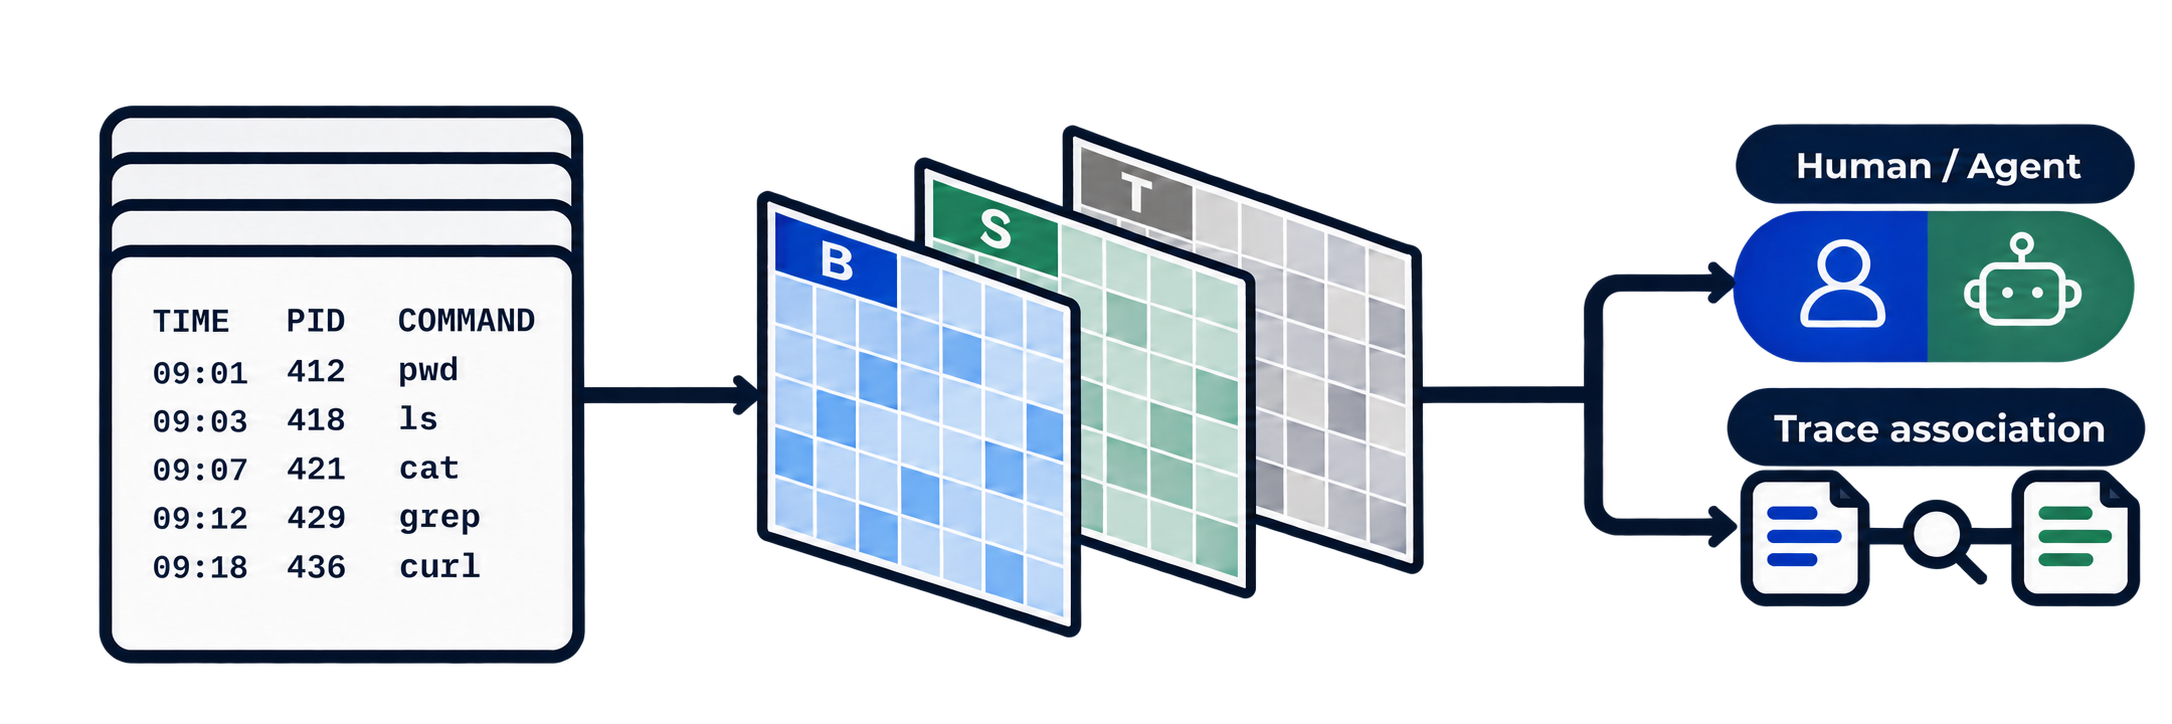
\includegraphics[width=\linewidth]{fingerprint-v3-overview.png}
\par\vspace{.15em}
\noindent\makebox[\linewidth][l]{%
\begin{minipage}[t]{.31\linewidth}\centering\small
\textbf{Observable logs}\\Commands, order, timing
\end{minipage}%
\begin{minipage}[t]{.38\linewidth}\centering\small
\textbf{B/S/T fingerprint}\\Behavior, sequence, timing
\end{minipage}%
\hspace{.09\linewidth}%
\begin{minipage}[t]{.22\linewidth}\centering\small
\textbf{Two readouts}\\Mode scoring; association
\end{minipage}%
}\par
\caption{From observable logs to a windowed behavioral fingerprint and two separately evaluated readouts. For the selected log trace, the three displayed sheets show the B, S, and T feature blocks; their columns form a single fingerprint matrix. The operation repeats for each trace before association. Timing remains missing when unavailable. Log fields and cell colors are illustrative, not measured values.}
\label{fig:architecture}
\end{figure}

The experiments connect this design to measurable utility. Evidence-conditioned B/S improves held-out association BA on two of three within-source cohorts (CTH and KYPO), while Antieval is unresolved. Entire-source holdouts produce one positive, one unresolved, and one negative change across those same sources. These are two protocols on three sources, not six independent datasets. CTH ablation measures the contribution beyond command evidence and length. AIT provides real launch times for a separate T-block and mode-recognition study; CTH, Antieval, and KYPO association views contain no comparable event timestamps, so their association models use B/S.

\paragraph{Contributions.} (1) A log-derived, variable-length B/S/T fingerprint with interpretable features and explicit missingness. (2) An evaluation of execution-mode composition and fingerprint contributions to recognition and association. (3) A multi-source evaluation and reproducible evidence record that characterize the representation across common log contracts and held-out conditions.

\section{Related work and positioning}
\paragraph{System identity and workflow.} Recent work shows that agent execution traces carry information about the system producing them, across terminal, coding, and browser interfaces. Trace classifies seven model families from terminal-command sequences collected with three scaffolds, then uses the predicted family to select a follow-on defensive prompt-injection probe~\cite{trace}. LIDAR instead actively issues controlled coding tasks and compares decision and action traces against enrolled model references across two harnesses~\cite{lidar}. Known By Their Actions studies passive identification from browser UI events and timing across four sites, including early-episode and open-set settings~\cite{known}. These studies establish identity and auditing readouts under their respective reference sets, interfaces, and interventions; the identity label is not a relation label between arbitrary traces. ProcGrep broadens the workflow view: it encodes coding-agent trajectories as procedures for agent fingerprinting, procedural comparison, and episodic search, rather than restricting analysis to individual command tokens~\cite{procgrep}. Together, these works motivate extracting behavior from logs while also showing why collection interface, available reference population, and task definition must accompany any claim of transfer.

\paragraph{Attack behavior and relation evidence.} CyBiasBench characterizes attack-selection preferences by measuring how five agents distribute effort across attack families under varied prompts, targets, and steering conditions~\cite{cybias}. This is evidence about behavioral tendencies at the agent level, rather than a method for linking two observed traces to a shared event or campaign. Cross-Agent addresses a closer relation-inference problem: it scores whether asynchronously observed sessions belong to a common campaign from proxy-visible structural, textual, and temporal residue, evaluated with controlled synthetic campaign labels~\cite{crossagent}. Its relation target and evidence channels therefore differ from both identity classification and the benchmark-task relation used here. Table~\ref{tab:related} summarizes these distinctions alongside the observation scope and whether each method passively reads logs or intervenes through task conditions or probes.

\paragraph{Positioning.} This study evaluates whether command-sequence and local behavior evidence can rank traces associated with the same benchmark task under held-out sources and changing recorded Human/Agent composition. The task label is a retrieval proxy: it does not establish common attack activity, campaign, operator, or Agent instance. Unlike identity classifiers, the association scorer does not require a catalogue covering every model family; unlike active identification, it uses retained traces without issuing new probes. Unlike Cross-Agent, it does not claim campaign attribution, and its relation labels are benchmark tasks rather than synthetic campaigns. The experiments therefore test a narrower but complementary question: how far passive trace evidence supports same-task retrieval under source-specific observation contracts. Table~\ref{tab:related} separates these objectives and requirements.

\begin{table}[ht]
\centering\compacttable
\caption{Related work by research objective, evaluated scope, observed evidence, and intervention. Candidate sets and task domains differ; Cross-Agent uses synthetic campaign labels.}\label{tab:related}
\begin{tabularx}{\linewidth}{@{}p{.26\linewidth}p{.15\linewidth}p{.20\linewidth}p{.17\linewidth}Y@{}}
\toprule
Work & Objective & Evaluated scope & Observation & Intervention \\
\midrule
\multicolumn{5}{@{}l}{\textit{System identity and workflow}} \\
\mbox{Trace~\cite{trace}} & Model family & 7 families; 3 scaffolds & Terminal commands & Active follow-on \\
\mbox{ProcGrep~\cite{procgrep}} & Workflow; search & 10 coding Agents & Coding actions & Passive \\
\mbox{LIDAR~\cite{lidar}} & Model identity & 36 models; 2 harnesses & Coding traces & Active probes \\
\mbox{Known By Their Actions~\cite{known}} & Browser model & 14 models; 4 sites & UI events; time & Passive \\
\midrule
\multicolumn{5}{@{}l}{\textit{Attack behavior and relation evidence}} \\
CyBiasBench~\cite{cybias} & Attack preference & 5 Agents; 3 targets & HTTP requests & Task conditions \\
\mbox{Cross-Agent~\cite{crossagent}} & Campaign links & Synthetic campaigns & Events; text; time & Logs and probes \\
This study & Trace association & 3 sources; 2 protocols & Command sequences & Passive \\
\bottomrule
\end{tabularx}
\end{table}

\paragraph{Association without a model-identity prerequisite.} Our fingerprint exposes differences between traces directly to a relation-trained scorer. The feature definition and association output do not require a catalogue covering every current model or Agent product, and inference uses retained logs rather than new probe executions. This makes the interface applicable to unidentified execution systems with compatible logs. Its empirical transfer is measured by held-out tasks, participants, and sources; the mixed source-holdout results bound that claim. Human/Agent recognition is a separately evaluated readout, not a prerequisite for association.

System behavior association offers a complementary foundation. ATLAS reconstructs attack stories from causal audit-graph sequences; HOLMES maps provenance evidence to attack stages and campaign signals; OSTINATO compares provenance-graph behavior across hosts; POIROT and SFM align threat-intelligence behavior with system records~\cite{atlas,holmes,ostinato,poirot,sfm}. These methods use richer process, object, causal, or attack-specific evidence than command-name sequences. The command-log fingerprint complements these process and provenance graph methods by operating on ordered event views and measured timing. Task-labelled retrieval supplies the relation contract for the present evaluation.

\section{Data and observation contracts}
The downloadable registry contains 1,407 source-qualified trace and task records from four source families. The bundle preserves separate source-specific cohorts and evaluation contracts. The experiments use the cohorts below, defined by relation labels, observed fields, minimum event counts, and held-out units. Honey and CyBiasBench are supplemental external-source analyses with their own upstream data access.

\begin{table}[ht]
\centering\compacttable
\caption{Cohort coverage. Green robot and blue person icons mark recorded Agent and Human counts; absent classes are omitted. Counts refer to records or sessions; external-source analyses are separate from the downloadable registry.}
\begin{tabularx}{\linewidth}{@{}p{.19\linewidth}p{.10\linewidth}p{.18\linewidth}p{.18\linewidth}Y@{}}
\toprule
Cohort & Records & Mode counts & Observable evidence & Task or evaluation \\
\midrule
Packaged registry & 1,407 & \mixedcounts{344}{1,063} & Command view & Catalog; not pooled \\
Original CTF & 97 & \mixedcounts{57}{40} & Commands; artifacts & 40 tasks; fixed pair panel \\
CTH mixed-mode & 175 & \mixedcounts{57}{118} & Command order & 40 tasks; cross-mode retrieval \\
CTH mixture core & 85 raw & \mixedcounts{34}{51} & Command order & 17 tasks; role mixtures \\
Antieval & 163 & \agentcount{163} & Command order & 32 tasks; Agent retrieval \\
KYPO & 197 & \humancount{197} & Command order & 97 people; task-level pairs \\
AIT audit logs & 109 & \mixedcounts{61}{48} & Launches; timing & 12 tasks; mode recognition \\
Honey~\cite{honey} & 13,080 & \agentcount{13,080} & Commands; duration & Same prompt/environment condition \\
CyBiasBench~\cite{cybias} & 450 & \agentcount{450} & HTTP method; route & Target and requested family \\
\bottomrule
\end{tabularx}
\end{table}

CTH provides the main Human/Agent same-task setting. Human sessions were captured through terminal recording, whereas Agent sessions use structured tool calls. A common challenge name provides shared task context but does not equalize capture interfaces, establish the same attack, or identify a common operator. The 40-task mixed cohort has 177 raw traces; two Agent traces do not meet the minimum two-command feature gate, leaving 175 eligible observations. The stricter 17-task mixture core retains at least two raw traces of each mode per task; 84 of its 85 raw records meet the fingerprint feature gate.

AIT is a troubleshooting benchmark, not an attack dataset. Its task and collection workflows co-vary with the released Human/Agent labels. We preserve a frozen 89-run comparison for continuity and include the complete 109-run eligible queue for an expanded analysis. Honey records command execution durations but not event start times; those durations are never treated as inter-command gaps. CyBiasBench has no precise time fields. Accordingly, T is omitted where unavailable.

\begin{table}[ht]
\centering\compacttable
\caption{Observed fields and evaluation role by source. A check marks an observed field; a dash marks an unavailable field. Honey execution duration is not treated as an event timestamp.}
\label{tab:observation-contracts}
\begin{tabularx}{\linewidth}{@{}p{.22\linewidth}p{.14\linewidth}p{.07\linewidth}p{.10\linewidth}p{.10\linewidth}p{.10\linewidth}Y@{}}
\toprule
Source & Unit & Order & Start time & Duration & Modes & Evaluation role \\
\midrule
CTH mixed tasks & 175 traces & \present & -- & -- & \mixedmodes & Same-task retrieval; exact role mixtures \\
AIT audit logs & 109 runs & \present & \present & -- & \mixedmodes & Mode recognition; observed launch rhythm \\
Honey for the Agent & 13,080 sessions & \present & -- & \present & \mbox{A\,\agenticon} & External-source command and duration analysis \\
CyBiasBench & 450 sessions & \present & -- & -- & \mbox{A\,\agenticon} & Target-held-out request retrieval \\
\bottomrule
\end{tabularx}
\end{table}

\section{Method: an interpretable B/S/T fingerprint}
\subsection{Representation}
An adapter maps each source to ordered event symbols, optional coarse action labels, and only the time fields that were actually observed. For sequence $x=(x_1,\ldots,x_n)$, we form consecutive windows of eight events and retain any final window meeting the source-specific minimum (two commands for the CTH mixture and four for AIT/Honey). At most the first 128 events are used. This removes the former sixteen-command admission gate. The number of valid windows $J$ varies across traces; unavailable measurements remain missing. We do not impose attack phases.

Each window yields three blocks:
\begin{itemize}[leftmargin=1.4em,itemsep=0.1em]
\item \textbf{B8, local behavior:} command-name diversity, command entropy, dominant-command share, coarse-action switching and transition entropy, longest action run, repeated action-pair share, and repeated-command adjacency.
\item \textbf{S8, sequence evolution:} first-seen command share, revisit share and revisit lag, action return motifs, action recurrence at lag three, reused command bigrams/trigrams, and change in the action distribution from the preceding window.
\item \textbf{T8, observed timing:} median and interquartile range of nonnegative inter-event gaps, burstiness, fractions of gaps at most one second and at least ten seconds, lag-one correlation of log gaps, median observed event duration, and median idle time after a completed event.
\end{itemize}
The local block uses the eight coarse command groups already defined by the repository adapter: discover, read, search, execute, build, network, modify, and environment. Timing features are calculated only from aligned timestamps or durations supplied by the source. No response-generation delay is relabelled as command spacing.
Figure~\ref{fig:bst-dimensions} brings all 24 measurements into one schematic atlas, grouped by B, S, and T and aligned by feature index.

The per-window matrix is $J\times16$ when B and S are available and $J\times24$ when timing is also observable. For fixed-dimensional classifiers, each feature column contributes its mean, population standard deviation, and least-squares trend across normalized window position: 48 values for B+S and 72 for B+S+T. This summary is a separate readout from the original 24-value static K1--K8 profile. Figure~\ref{fig:matrix} displays actual AIT windows; hatched gray cells indicate unavailable observations.

\begin{figure}[ht]
\centering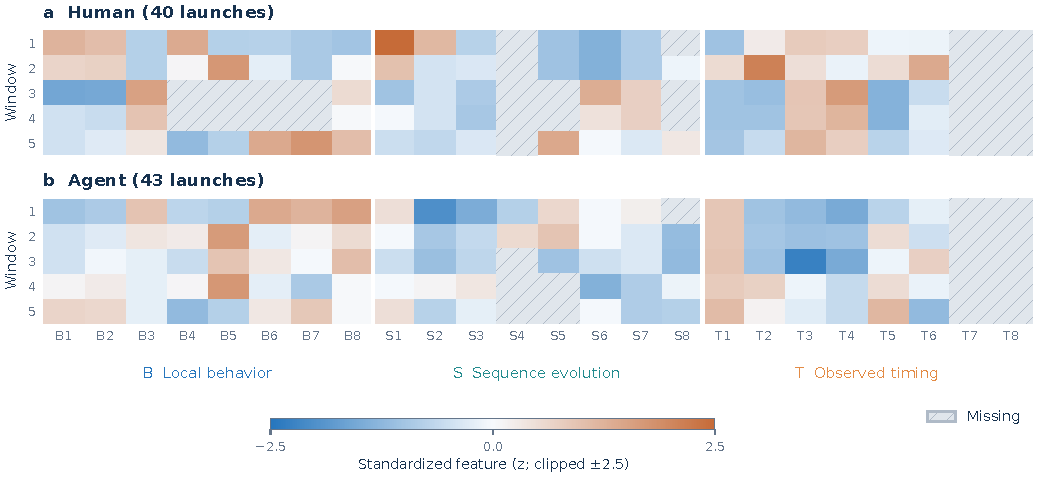
\includegraphics[width=\linewidth]{fingerprint-v2-matrix-example.pdf}
\caption{Two real AIT traces for the same troubleshooting task, visualized as 24 columns (B, S, T) over variable-length windows. A shared blue--amber scale shows cohort-standardized values for display only; hatched cells mark missing fields.}
\label{fig:matrix}
\end{figure}

\subsection{Two readouts}
\textbf{Execution-mode readout.} Regularized logistic regression predicts the released Human/Agent label from the fixed-dimensional summaries; a fixed shallow ExtraTrees model is a nonlinear comparison. Baselines include length, command TF--IDF, and the old eight-feature profile. Task groups are held out. In the AIT source-holdout panel, task families remain represented across folds, so it is a source-group stress test rather than independent cross-domain validation.

\textbf{Pairwise association readout.} For CTH cross-mode retrieval, command TF--IDF cosine is compared with a regularized pair classifier using command cosine and negative train-standardized L1 distances for B and S. T is excluded because the CTH command view has no timestamps. The classifier is trained on other task groups only; both query and candidate task groups are held out from model fitting. In the role-mixture baseline, command and action-bigram cosine scores use thresholds selected on training-side task-held-out predictions by maximizing recall subject to a false-merge rate of at most 10\%. We report both ranking metrics and thresholded errors; they answer different questions.

\subsection{Evidence-conditioned tree association}
For the exploratory BA study, the shared evidence vector $E$ contains command TF--IDF cosine and coarse-action bigram cosine. Each trace has a train-standardized 48-value B/S summary $z$. The fingerprint model adds the component-wise interaction $E_{\mathrm{cmd}}|z_i-z_j|$ to $E$, so the classifier can learn how each behavioral difference changes the interpretation of command evidence. We compare it with the same learner trained on $E$ alone, using identical training pairs, test candidates, and training-side threshold selection. The learner is a 64-tree ExtraTrees classifier with a minimum leaf size of three; depth is selected from 3, 5, and 8 in inner validation. Feature imputation, scaling, and vocabulary are fit on training records only. Tree-path probability changes are grouped by evidence, B, and S and sum exactly to each model score; these are model explanations rather than causal effects.

\begin{figure}[ht]
\centering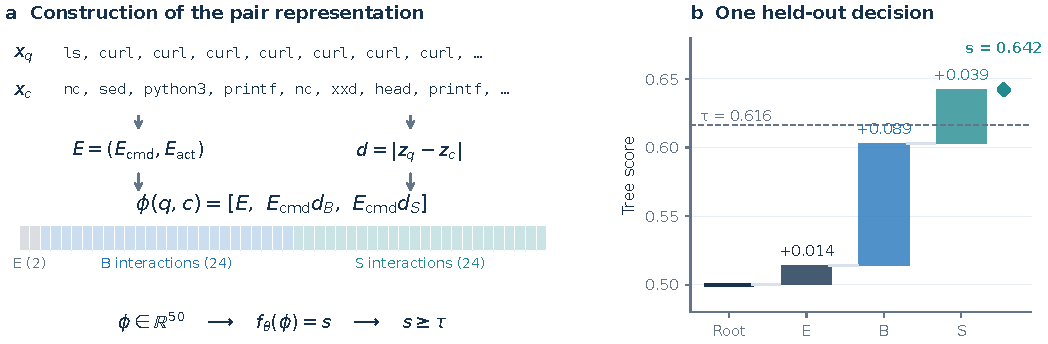
\includegraphics[width=\linewidth]{fingerprint-conditioned-association.pdf}
\caption{Conditioned association and one held-out CTH \texttt{locktalk} decision. (a) The first eight commands of each trace illustrate one window; two evidence values and 48 command-conditioned B/S differences enter the tree scorer. Vector partitions are schematic. (b) Exact score contributions for the median acceptance margin among 31 cross-mode same-task pairs corrected in the purged source holdout. Each model uses its own training-selected threshold. Contributions explain the fitted model score rather than calibrated link probability or causality.}
\label{fig:conditioned-association}
\end{figure}

The example in Figure~\ref{fig:conditioned-association} makes the evidence path inspectable: the evidence-only score is 0.579 at threshold 0.609, whereas the conditioned score is 0.642 at threshold 0.616. The latter decomposes into a 0.500 root, $+0.014$ evidence, $+0.089$ B, and $+0.039$ S contributions. These are contributions within the fitted full model, not a decomposition of its difference from the evidence-only model. The task and execution-mode labels describe the example and are not input features.

The external-source retrievals use source-specific event views and labels. Honey positives share prompt, turn cap, and environment but differ by held-out model snapshot; its duration ablation uses observed execution-duration fields. CyBiasBench uses request method and normalized route sequence, while target and requested-family fields define evaluation conditions only. Neither source supplies real actor or campaign identity.


\section{Experimental protocol}
\subsection{CTH role mixtures}
The 17-task core is split by challenge group into the existing three outer folds. Each of 170 paired allocations rotates one excluded task and selects one query and one gallery trace for each of the remaining 16 tasks. Of the resulting 32 role slots, exactly 0, 8, 16, 24, or 32 are assigned Agent traces, giving 0, 25, 50, 75, and 100\% Agent roles. Each query is compared with its same-task candidate and three different-task candidates from the same held-out fold. The candidate tasks and role allocations are coupled across the five proportions; both baseline methods share the same draws. Thresholds are selected on training tasks and held fixed across proportions within each fold. We average repeated allocations within each task before resampling the 17 task groups for uncertainty intervals.

\subsection{All-task cross-mode retrieval}
We use all 40 CTH tasks containing at least one feature-eligible trace of each mode (175 traces: 57 Human and 118 Agent). Five outer folds hold out eight task groups at a time. Each held-out query is matched against one opposite-mode gallery trace from each of the eight held-out tasks. Thus the gallery contains one same-task proxy and seven different-task candidates (chance Hit@1 = 12.5\%). The trained score sees only the other 32 tasks. We report both Human-to-Agent and Agent-to-Human query directions and task-cluster bootstrap intervals over 40 tasks.

\subsection{BA comparison and source holdout}
The post-observation BA study uses five task-group folds on 175 CTH traces, three task-group folds on 163 Antieval traces, and five participant-disjoint folds on 197 KYPO traces. The held-out Antieval gallery evaluates 31 task groups and the KYPO panel evaluates 190 queries. In each outer fold, three inner folds choose tree depth, decision threshold, and a B/S window of 4, 8, or 16 events. The evidence-only comparison uses the same learner and candidates. We resample 40 CTH tasks, 31 Antieval tasks, or 97 KYPO query participants after averaging repeated observations. KYPO candidate galleries remain fixed under query-participant resampling.

For the CTH ablation, we instead fix the B/S window at eight events and compare the full model with block removals and a length-only control on the same outer galleries. The leave-one-source-out study holds out CTH, Antieval, or KYPO entirely. Models train on source-balanced, same-source task pairs from the remaining sources, and two inner source holdouts select depth and threshold. The B/S window is fixed at eight events. Where CTH and Antieval share a normalized CyBench challenge name, training records with that name are purged against both outer and inner validation sources; 33 and 26 training records are removed when holding out CTH and Antieval, respectively. Each test query is compared with one same-task and seven different-task candidates. Source and task labels determine splits and pairs, not the feature vector. These analyses were specified after inspecting prior results; reported intervals are unadjusted exploratory intervals.

\subsection{AIT recognition and supplemental sources}
For AIT, we compare frozen 89-run and expanded 109-run cohorts under task-group and source-group holdouts. Feature scaling and imputation are fit on training folds only. Paired changes add S to B and then T to B+S. We also compare full B+S with a fixed first eight-event window, shuffled eight-event window order, and B+S+T with observed gaps permuted within each eight-event window. Twenty perturbations are averaged per trace; task-cluster intervals resample the 12 task groups. These controls diagnose the AIT cohort and do not isolate mode from workflow. For Honey, query/candidate conditions are fixed and the held-out model snapshot is varied; 10,368 queries are summarized over 48 prompt/cap/environment clusters. For CyBiasBench, one target application is held out at a time; there are 600 queries per target with one positive and four negatives. Because there are only three targets, we report per-target range rather than a query-level confidence interval.

\section{Results}
\subsection{Exact role mixtures revisit the baseline hypothesis}
We retain the original 17-task core, its outer task folds, and the training-side FMR-at-most-10\% threshold. In each of 170 coupled allocations, 16 tasks contribute 32 query/gallery roles; the excluded task rotates evenly. Exactly 0, 8, 16, 24, or 32 roles are Agent, and candidate tasks are coupled across concentrations. Each query has one same-task and three different-task candidates. The command baseline BA declines from 53.6\% to 46.5\% ($-7.10\pp$; 95\% task-cluster interval $[-15.45,+0.06]$), while action-bigram BA declines from 57.4\% to 46.5\% ($-10.92\pp$ $[-20.61,-3.06]$). Between the endpoints, FSR rises while FMR falls. This rerun changes the candidate count from five in the older approximate-share experiment and remains a task-proxy evaluation.
\begin{figure}[ht]
\centering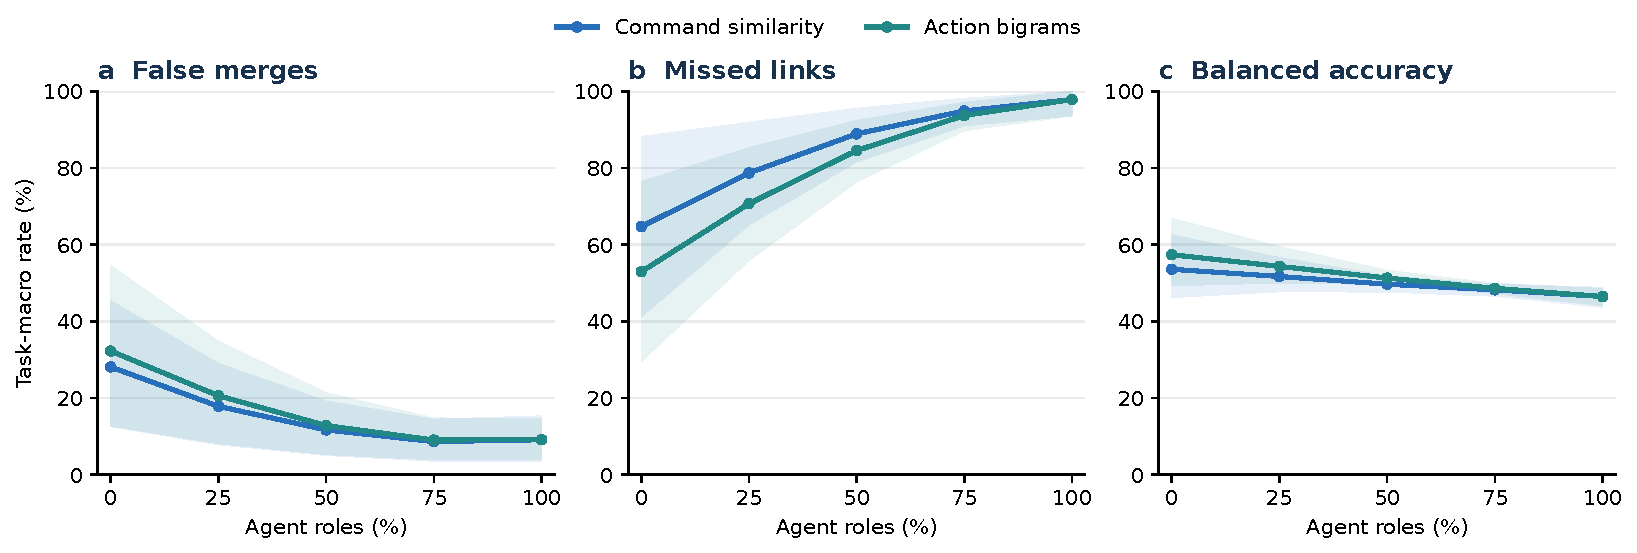
\includegraphics[width=\linewidth]{exact-mixture-v3.pdf}
\caption{Exact role-mixture baseline rerun: FMR, FSR, and BA in three aligned panels. Shading resamples the 17 task groups after averaging paired allocations within each task.}
\label{fig:exact-mixture}
\end{figure}

\subsection{Conditioned fingerprints improve held-out association}
Conditioning command evidence on B/S increases same-task association BA in the CTH and KYPO comparisons. With identical learners, training pairs, and test galleries, CTH improves from 65.07\% to 68.00\% ($+2.94\pp$, 95\% paired interval $[+0.43,+5.34]$), and KYPO from 55.83\% to 60.08\% ($+4.25\pp$, $[+1.03,+8.02]$). Antieval changes from 70.24\% to 70.38\% ($+0.13\pp$, $[-2.47,+2.61]$). Figure~\ref{fig:association-comparison} shows all three within-source comparisons, with task or participant holdout and training-side window selection.

\begin{figure}[ht]
\centering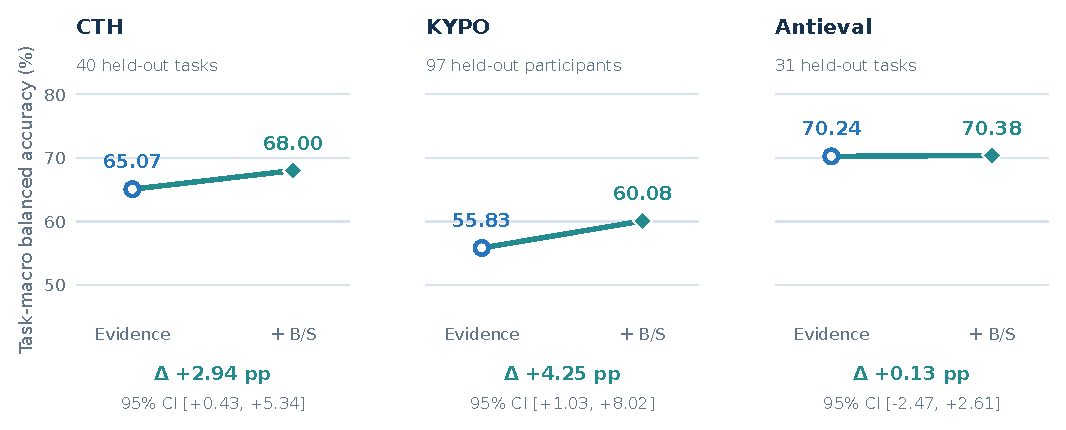
\includegraphics[width=\linewidth]{fingerprint-association-comparison.pdf}
\caption{Evidence-conditioned association on all three within-source cohorts. Panel a compares the same shallow-tree family before and after adding B/S; panel b reports paired BA differences and 95\% cluster intervals. CTH and Antieval resample tasks; KYPO resamples query participants with galleries fixed. These post-observation intervals are exploratory and unadjusted.}
\label{fig:association-comparison}
\end{figure}

Holding out an entire log source tests a stronger change in observation conditions. The source-held-out CTH model gains $4.71\pp$ in BA, and its FSR falls from 85.8\% to 72.9\%, accompanied by an FMR increase from 10.3\% to 13.7\%. KYPO changes by $+0.21\pp$ and Antieval by $-3.27\pp$ (Table~\ref{tab:association-ba-v3}). The source-held-out result therefore depends on the input contract: the CTH gain transfers to a new source, while the Antieval comparison records a loss. Known matching CyBench challenge names are purged from both outer and inner training sources.

\begin{table}[ht]
\centering\compacttable
\caption{Complete source-held-out association comparison. Training uses the other sources; B/S windows contain eight events. BA is in percent; differences and unadjusted 95\% cluster intervals are in percentage points. Green/red encode improvement/decline in the point estimate; interval bounds retain the uncertainty.}
\label{tab:association-ba-v3}
\setlength{\tabcolsep}{3pt}
\begin{tabular*}{\linewidth}{@{\extracolsep{\fill}}lrrr@{}}
\toprule Test source & Evidence & + B/S & $\Delta$BA [95\% CI] \\
\midrule
CTH & 51.98 & 56.69 & $\gain{+4.71}\;\textcolor{ResearchMuted}{[+0.69,+8.83]}$ \\
KYPO & 66.40 & 66.61 & $\gain{+0.21}\;\textcolor{ResearchMuted}{[-1.06,+1.36]}$ \\
Antieval & 71.90 & 68.63 & $\loss{-3.27}\;\textcolor{ResearchMuted}{[-6.28,-0.22]}$ \\
\bottomrule
\end{tabular*}
\end{table}

\subsection{Feature-block ablation on held-out CTH tasks}
We isolate the fingerprint contribution on 175 traces from 40 mixed-mode CTH tasks. All rows use the same outer task folds, query--candidate galleries, evidence features, and shallow-tree family. Each model selects its depth and decision threshold on inner training tasks. The full configuration combines command and action-bigram evidence with command-conditioned B and S feature differences, using fixed eight-event windows. The length control adds only the log-length difference to the same evidence; the two ablations retain only S or only B, respectively. T is unavailable in this CTH command view and is evaluated separately on AIT.

\begin{table}[ht]
\centering\compacttable
\caption{CTH fingerprint ablation. BA is task-macro balanced accuracy (\%); $\Delta$ compares each row with the full B/S model in percentage points. Intervals resample the 40 paired task-level outcomes 10,000 times; they are exploratory and unadjusted for multiple comparisons.}
\label{tab:fingerprint-ablation}
\setlength{\tabcolsep}{3pt}
\begin{tabular*}{\linewidth}{@{\extracolsep{\fill}}lccrr@{}}
\toprule Configuration & B & S & BA (\%) & $\Delta$ vs. full [95\% CI] \\
\midrule
Evidence only & -- & -- & 65.07 & $\loss{-2.03}\;\textcolor{ResearchMuted}{[-3.98,-0.08]}$ \\
Evidence + length & -- & -- & 65.78 & $\loss{-1.32}\;\textcolor{ResearchMuted}{[-4.12,+1.49]}$ \\
Remove B & -- & \present & 63.96 & $\loss{-3.14}\;\textcolor{ResearchMuted}{[-6.21,-0.22]}$ \\
Remove S & \present & -- & 65.63 & $\loss{-1.46}\;\textcolor{ResearchMuted}{[-4.21,+1.07]}$ \\
\midrule
\textbf{Full B/S} & \present & \present & \gain{\textbf{67.10}} & Reference \\
\bottomrule
\end{tabular*}
\end{table}

Removing B reduces BA by $3.14\pp$ relative to the full model in this fixed-window comparison; removing S reduces the point estimate by $1.46\pp$, with an interval spanning zero. The length-only control also has an interval spanning zero relative to the full model. The fixed-window comparison identifies B as the clearest measured block contribution; the S and length contrasts retain wider uncertainty. The full-model BA here differs from the nested-window CTH result in Figure~\ref{fig:association-comparison} because the ablation fixes the window at eight events.

\subsection{Timing adds an interpretable execution-mode signal}
On the complete 109-run AIT cohort, the linear B+S+T readout reaches 68.8\% task-macro BA, compared with 53.0\% for B+S. The paired gain is $+15.83\pp$ (95\% task-cluster interval $[+6.11,+25.00]$). Under source-group holdout, adding T raises BA from 35.8\% to 52.6\% ($+16.88\pp$, $[+8.19,+25.77]$). Figure~\ref{fig:recognition} compares all seven readouts on these same 109 runs. The source-group absolute score remains close to 50\%, and task families remain shared across folds. The frozen 89-run comparison is reported in Appendix~\ref{app:recognition}.

\begin{figure}[ht]
\centering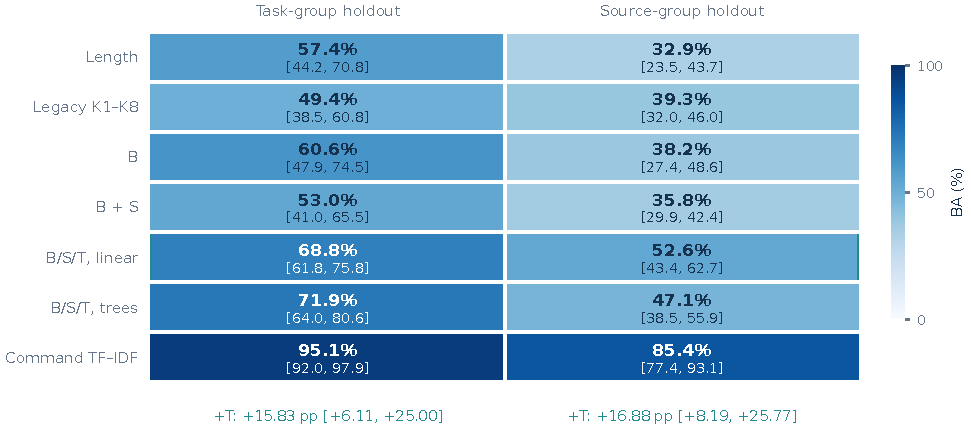
\includegraphics[width=\linewidth]{fingerprint-recognition-matrix.pdf}
\caption{Recognition as a feature-by-holdout performance matrix on all 109 eligible AIT runs (61 Human, 48 Agent; 12 task groups). Cells show task-macro BA and 95\% task-cluster intervals on fixed out-of-fold predictions. The outlined row is the linear B/S/T readout; the bottom annotations are its paired T increment. Vocabulary is a separate baseline; collection workflows co-vary with the released labels.}
\label{fig:recognition}
\end{figure}

The time block measures concrete launch structure. Figure~\ref{fig:timing} links the same two real Nextcloud traces used in the fingerprint matrix to the distribution across all 109 runs. The median of per-run median launch gaps is 0.553 seconds for Human-labelled runs and 9.007 seconds for Agent-labelled runs. These values describe login-associated process launches in this collection, including script-generated launches; the distribution gives each run one observation. This connects T to a measurable log property while keeping workflow and execution mode jointly visible.

\begin{figure}[ht]
\centering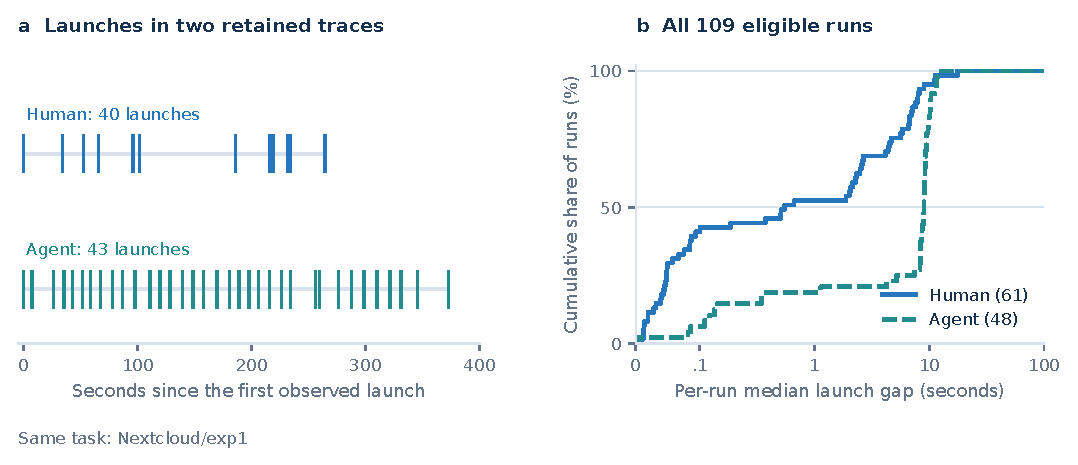
\includegraphics[width=\linewidth]{fingerprint-observed-rhythm.pdf}
\caption{Observed timing behind T. Left: real launch timestamps from the same Human and Agent traces as Figure~\ref{fig:matrix}, aligned to their own first observed launch with a shared seconds scale. Right: empirical cumulative distributions of one median launch gap per run over the complete 109-run cohort, with the two group medians marked, with a zero-preserving logarithmic seconds scale above 0.1 seconds. At most the first 128 login-associated events are retained; zero gaps are included. The trace pair illustrates the measurement; the full-cohort panel describes its distribution.}
\label{fig:timing}
\end{figure}

\paragraph{Controls locate the predictive information.} Table~\ref{tab:ait-controls} replaces a repeated score plot with explicit interventions. Using the first eight events gives 72.3\% task-held-out BA, compared with 53.0\% for full B+S ($+19.3\pp$, $[+6.2,+31.9]$); the corresponding source-group gain is $+5.6\pp$ $[-2.8,+12.9]$. Shuffling window order produces 55.8\% task-held-out BA. Permuting observed gap order within each window preserves the local gap distribution and gives 70.6\% for B+S+T, compared with 68.8\% before permutation. These controls locate useful information in workflow prefixes and per-window gap summaries; they provide little support for a distinct benefit from the tested fine-order summaries.

\begin{table}[ht]
\centering\compacttable
\caption{AIT feature controls, 109 runs. BA (\%) and 95\% task-cluster intervals are shown for both holdouts. Shuffled controls average 20 perturbations per trace.}
\label{tab:ait-controls}
\setlength{\tabcolsep}{3pt}
\begin{tabularx}{\linewidth}{@{}Yrr@{}}
\toprule Configuration & Task-group BA [95\% CI] & Source-group BA [95\% CI] \\
\midrule
B+S, full trace & $53.0\;[41.0,65.5]$ & $35.8\;[29.9,42.4]$ \\
B+S, first eight events & $72.3\;[64.9,79.0]$ & $41.4\;[33.7,48.4]$ \\
B+S, window order shuffled & $55.8\;[49.7,61.7]$ & $40.3\;[31.9,48.6]$ \\
B+S+T, full trace & $68.8\;[61.8,75.8]$ & $52.6\;[43.4,62.7]$ \\
B+S+T, gap order shuffled & $70.6\;[61.9,79.5]$ & $49.9\;[44.1,55.9]$ \\
\bottomrule
\end{tabularx}
\end{table}

\subsection{Ranking and observation contracts delimit the use of each readout}
The association BA improvements concern decisions at training-selected thresholds. The opposite-mode CTH ranking comparison remains effectively unchanged: command cosine gives 33.65\% Hit@1 and 0.539 MRR, while the linear command+B/S score gives 33.56\% and 0.535 ($\Delta$Hit@1 $-0.08\pp$, $[-5.71,+5.58]$). Thus the current utility is a learned association decision and its interpretable component evidence, rather than a demonstrated general increase in top-one retrieval.

SSH, HTTP, and Human-only cohorts test different observation contracts. Honey's B/S retrieval change is $-1.30\pp$ $[-2.21,-0.35]$; adding its observed execution durations changes Hit@1 by $-0.35\pp$ $[-0.87,+0.16]$. KYPO's linear ranking fusion changes Hit@1 by $-1.42\pp$ $[-2.59,-0.23]$. CyBiasBench's route+B/S score changes target-macro Hit@1 by $+0.92\pp$, with per-target differences from $-0.17$ to $+1.58\pp$. Its FMR falls from 13.6\% to 2.8\% as FSR rises from 74.7\% to 92.8\%, reducing BA from 55.9\% to 52.2\%. These comparisons retain their source-specific labels and fixed cohorts. Appendix~\ref{app:transfer} provides the complete table, including the legacy profiles and original artifact baseline; Appendix~\ref{app:refinement} records all fusion and alignment attempts.

\section{Discussion and limitations}
\paragraph{Implications for behavioral association.} In the evaluated five-level allocation, the fixed training-selected threshold accepts fewer same-task and different-task links as Agent-role share rises. Lower FMR and higher FSR therefore describe a more conservative operating point, with missed links dominating the decline in BA. Execution composition can change how a behavioral score should be used for a decision. The fingerprint supplies explicit tool-organization, repetition, sequence, and optional timing measurements for that decision. The source-held-out CTH fusion recovers some same-task links with additional false merges, so its benefit is the measured error tradeoff at the stated threshold. Capture differences remain part of the observed pattern.

\paragraph{Observation determines feature value.} AIT timing provides the clearest positive fingerprint increment. Its first-window and gap-order controls indicate where that signal resides. The command-only CTH panel and external retrieval panels show that richer structure alone does not ensure higher rank accuracy. Future extensions should connect the feature block to the relation being scored and preserve the source's time semantics.

\paragraph{Scope and validation.} Relation labels are benchmark tasks or source-specific conditions. Independently verified attack-activity, campaign, and operator labels are outside the current data. CTH terminal capture differs from Agent tool-call capture; AIT labels co-vary with troubleshooting workflows and collection sources. Honey and CyBiasBench contain Agent-only records. A separate broader-training mixture analysis showed a different, nonmonotonic baseline BA pattern, and its fingerprint BA gains had intervals crossing zero; the trend in Figure~\ref{fig:exact-mixture} should therefore be read in its specific allocation and training context. The datasets informed development and several alternatives were inspected before the tree study, so its intervals and nested refinements are exploratory and unadjusted for multiple comparisons. Known matching CyBench names are purged in the source holdout; unrecognized task or environment overlap can remain. KYPO query-participant resampling conditions on the selected galleries. Cross-source coverage establishes tested input contracts; matched collection and independent relations are required to extend the empirical claims to operational attack linkage.

\section{Conclusion}
Agent participation motivates reassessing the decision meaning of behavioral similarity. In our controlled CTF allocation, more Agent roles produce fewer false merges and more missed links, lowering BA at the fixed threshold. We make these execution differences available through an interpretable B/S/T fingerprint whose association branch uses trace-pair evidence without first identifying a named model or Agent product. B/S improves exploratory BA on two of three within-source cohorts; whole-source transfer improves CTH, leaves KYPO unresolved, and reduces Antieval BA. B contributes the clearest CTH block-ablation signal, while observed timing contributes to AIT mode recognition. The common representation supports logs from unidentified systems with compatible fields, and the source-specific results state where its present utility has been demonstrated. Extending that utility to independently verified attack activities remains a separate validation step.

\appendix
\section{Feature definitions and missingness}
{\compacttable
\begin{longtable}{@{}p{0.08\linewidth}p{0.22\linewidth}p{0.62\linewidth}@{}}
\caption{Window-level feature definitions. A value is missing when its required observations are absent or insufficient.}\label{tab:features}\\
\toprule Block & ID & Measurement \\
\midrule\endfirsthead
\toprule Block & ID & Measurement \\
\midrule\endhead
B & B1--B3 & Distinct command share; Shannon entropy of command names; share of the dominant command. \\
B & B4--B6 & Fraction of known adjacent action pairs that switch group; conditional entropy of the next action; longest single-action run divided by window length. \\
B & B7--B8 & One minus the unique mapped adjacent-action-pair share; fraction of adjacent command names that are identical. \\
S & S1--S3 & First-seen command share; fraction of repeated commands whose previous occurrence is at least two positions back; mean normalized log revisit span. \\
S & S4--S5 & A-B-A action return share among valid triplets; share of valid four-action segments whose first and fourth action match. \\
S & S6--S8 & Reused adjacent command-bigram share; reused command-trigram share; Jensen--Shannon divergence between current and preceding window action distributions. \\
T & T1--T3 & Median log(1+gap); interquartile range of log gaps; burstiness $(\sigma-\mu)/(\sigma+\mu)$ over nonnegative raw gaps. \\
T & T4--T6 & Fraction of gaps at most one second; fraction at least ten seconds; lag-one correlation of log gaps when at least three valid gaps exist. \\
T & T7--T8 & Median log(1+observed event duration); median log(1+idle interval) after subtracting observed duration from the next start time. \\
\bottomrule
\end{longtable}
}

\begin{figure}[ht]
\centering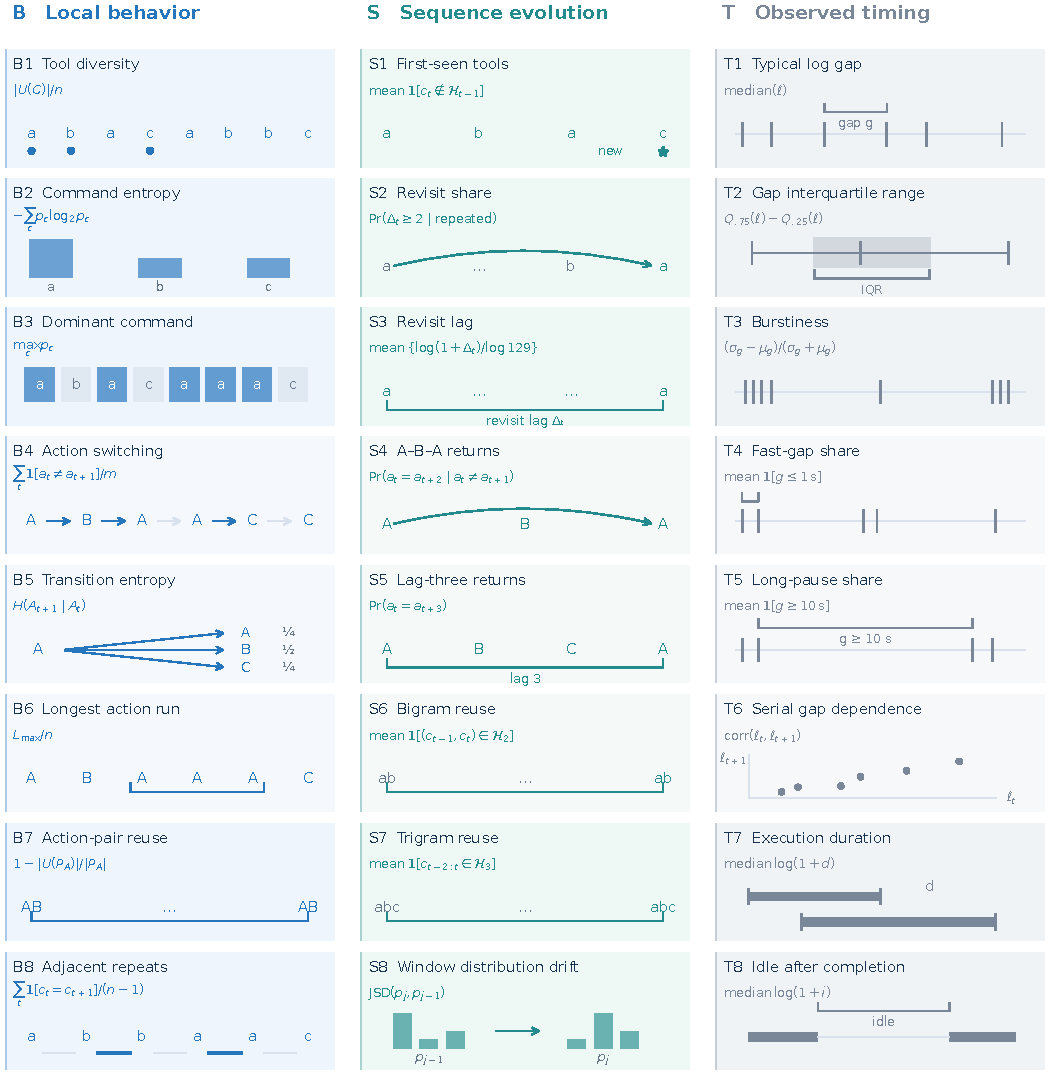
\includegraphics[width=\linewidth]{fingerprint-bst-dimensions.pdf}
\caption{The 24 B/S/T measurements, using the block colors of Figure~\ref{fig:architecture}. Glyphs illustrate definitions rather than measured results. Lowercase symbols denote commands and uppercase symbols coarse actions; $n$ counts window events, $m$ valid adjacent action pairs, $U$ unique values, $\mathcal{H}$ prefix history, and $\Delta_t$ revisit lag. For observed timing, $g$ is a nonnegative gap in seconds, $\ell=\log(1+g)$, $d$ duration, and $i$ nonnegative idle time.}
\label{fig:bst-dimensions}
\end{figure}

\section{Reproduction, versions, and data handling}
The fingerprint implementation is \texttt{attackagent/fingerprint\_v2.py}. Experiment scripts, fixed splits, predictions, and figure sources are organized under \texttt{research/experiments/} and \texttt{research/results/}, in the \texttt{behavioral\_fingerprint\_v2} and \texttt{association\_fingerprint\_v3} directories. Stored pair scores include thresholds and evidence-block contributions for reproducing the reported comparisons.

The 1,407-record download preserves source revisions, task keys, and licensing metadata; source terms apply separately. Honey and CyBiasBench use pinned snapshots with aggregate analyses, without redistributing modified CyBiasBench session rows. The original 97-trace panel remains separate from the expanded CTH cohort.

\section{Complete ranking and transfer comparisons}\label{app:transfer}
The additional experiments use their stated source-specific relation, observation, and holdout contracts. Their full results are retained independently of the primary within-source BA comparisons. Sample eligibility follows the field and task requirements in Section~3.

\begin{table}[ht]
\centering\compacttable
\caption{Additional transfer comparisons. Each row uses its stated outcome and held-out unit; changes are percentage points. The CyBiasBench interval is the range across three targets, not a confidence interval. Legacy denotes the earlier 24-value profile.}
\label{tab:transfer}
\setlength{\tabcolsep}{3pt}
\begin{tabularx}{\linewidth}{@{}p{.15\linewidth}p{.18\linewidth}Yp{.27\linewidth}@{}}
\toprule Source / $n$ & Holdout & Comparison; outcome & $\Delta$ [95\% CI] \\
\midrule
CTH / 175 & Task; opposite mode & Command $\to$ +B/S; Hit@1 & $\loss{-0.08}\;\textcolor{ResearchMuted}{[-5.71,+5.58]}$ \\
CTH / 219 & Task; Agent-only & Command $\to$ legacy; Hit@1 & $\loss{-3.57}\;\textcolor{ResearchMuted}{[-6.82,-0.43]}$ \\
AIT / 109 & Task & B/S $\to$ B/S/T; BA & $\gain{+15.83}\;\textcolor{ResearchMuted}{[+6.11,+25.00]}$ \\
AIT / 109 & Source group & B/S $\to$ B/S/T; BA & $\gain{+16.88}\;\textcolor{ResearchMuted}{[+8.19,+25.77]}$ \\
Honey / 13,080 & Model snapshot & Command $\to$ B/S; Hit@1 & $\loss{-1.30}\;\textcolor{ResearchMuted}{[-2.21,-0.35]}$ \\
CyBias / 450 & Target & Route $\to$ +B/S; Hit@1 & $\gain{+0.92}$; $\textcolor{ResearchMuted}{[-0.17,+1.58]}^\dagger$ \\
KYPO / 197 & Participant & Command $\to$ +B/S; Hit@1 & $\loss{-1.42}\;\textcolor{ResearchMuted}{[-2.59,-0.23]}$ \\
Antieval / 120 & Task & Command $\to$ legacy; Hit@1 & $\loss{-2.89}\;\textcolor{ResearchMuted}{[-7.50,+1.79]}$ \\
\bottomrule
\end{tabularx}
\end{table}

The earlier fixed 97-trace CTF panel evaluates command and distinctive-artifact evidence: Hit@1 rises from 29.60\% to 79.31\% and task-macro BA from 57.35\% to 62.06\%, with FMR 75.87\%. Its input, fixed pairs, and artifact score are distinct from the B/S study. In the 175-trace opposite-mode gallery, B-only and B+S standalone scores give 24.4\% and 26.1\% Hit@1. Command directional Hit@1 is 36.3\% for Human-to-Agent and 33.2\% for Agent-to-Human; command+B/S gives 33.8\% and 33.3\%.

The KYPO ranking panel uses 190 queries from 97 participants across eight task levels, with one same-task and four other-task candidates. Query and candidate participants differ. Command Hit@1 is 31.71\% and linear command+B/S is 30.29\%. Honey uses 10,368 queries over 48 prompt/cap/environment clusters; CyBiasBench has three held-out targets with 600 query draws each. CyBiasBench's target range is descriptive, while the other intervals use their stated cluster units.

\section{Frozen AIT recognition comparison}\label{app:recognition}
The 89-run cohort is retained for continuity. The complete 109-run cohort supplies the main performance matrix and all 109-run feature controls. On frozen AIT, adding T to B+S raises task-held-out BA by $15.1\pp$ $[+3.3,+26.7]$; the source-group paired interval spans zero. Table~\ref{tab:recognition-frozen} reports all seven frozen readouts.

\begin{table}[ht]\centering\compacttable
\caption{Frozen 89-run AIT readouts: task-macro BA (\%) and 95\% task-cluster intervals.}\label{tab:recognition-frozen}
\begin{tabularx}{\linewidth}{@{}Yrr@{}}\toprule Readout & Task-group holdout & Source-group holdout \\
\midrule
Length & $46.6\;[32.4,60.1]$ & $39.5\;[22.7,57.2]$ \\
Legacy K1--K8 & $55.2\;[45.6,66.2]$ & $44.9\;[33.4,56.1]$ \\
B & $56.3\;[40.9,71.6]$ & $39.9\;[25.6,54.2]$ \\
B+S & $55.5\;[45.6,65.6]$ & $39.6\;[28.5,50.8]$ \\
B+S+T (linear) & $70.6\;[63.6,78.5]$ & $44.4\;[31.7,54.7]$ \\
B+S+T (trees) & $73.0\;[63.1,82.4]$ & $44.9\;[32.8,56.7]$ \\
Command TF--IDF & $96.8\;[94.3,99.2]$ & $82.6\;[69.4,92.8]$ \\
\bottomrule\end{tabularx}\end{table}

\section{Complete refinement comparison}\label{app:refinement}
\begin{table}[ht]\centering\compacttable
\caption{Post-observation refinement on the identical 40-task, 175-query CTH galleries. Model family and regularization selection use inner tasks. All point estimates and paired task-cluster intervals are retained.}
\begin{tabularx}{\linewidth}{@{}YrrY@{}}\toprule Method & Hit@1 (\%) & MRR & $\Delta$Hit@1 [95\% interval], pp \\
\midrule
Command cosine & 33.65 & .539 & Reference \\
Scalar fusion, inner-selected C & 34.19 & .540 & $\gain{+0.54}\;\textcolor{ResearchMuted}{[-4.67,+5.88]}$ \\
Conditional B/S fusion & 30.02 & .518 & $\loss{-3.63}\;\textcolor{ResearchMuted}{[-9.13,+1.29]}$ \\
48 component differences & 23.92 & .453 & $\loss{-9.73}\;\textcolor{ResearchMuted}{[-19.00,-0.87]}$ \\
Local masked DTW fusion & 32.44 & .530 & $\loss{-1.21}\;\textcolor{ResearchMuted}{[-7.54,+5.08]}$ \\
Nested family selector & 33.35 & .537 & $\loss{-0.29}\;\textcolor{ResearchMuted}{[-5.67,+5.21]}$ \\
Command + cross-fitted mode & 30.52 & .518 & $\loss{-3.13}\;\textcolor{ResearchMuted}{[-9.17,+2.21]}$ \\
Command+B/S + cross-fitted mode & 31.15 & .522 & $\loss{-2.50}\;\textcolor{ResearchMuted}{[-9.13,+3.67]}$ \\
\bottomrule\end{tabularx}\end{table}
Mode assistance uses B/S summaries to predict mode, with three training-task folds supplying out-of-fold mode scores for association training. Outer-test mode scores use only the outer-training fit. True test mode labels remain evaluation metadata. KYPO intervals resample held-out query participants and recompute the available-task macro.

\begin{thebibliography}{99}
\bibitem{trace} Murali Ediga and Sudipta Chattopadhyay. ``Trace: Unmasking AI Attack Agents Through Terminal Behavior Fingerprinting.'' arXiv:2605.01186, 2026. \url{https://arxiv.org/abs/2605.01186}
\bibitem{procgrep} Hamidah Oderinwale. ``Agent Trajectories as Programs: Fingerprinting and Programming Coding-Agent Behavior.'' arXiv:2606.16988, 2026. \url{https://arxiv.org/abs/2606.16988}
\bibitem{lidar} Chuyi Wang et al. ``Who Is Behind the Harness? Fingerprinting LLMs through Agentic Behavior.'' arXiv:2609.28559, 2026. \url{https://arxiv.org/abs/2609.28559}
\bibitem{known} William Lugoloobi et al. ``Known By Their Actions: Fingerprinting LLM Browser Agents via UI Traces.'' arXiv:2605.14786, 2026. \url{https://arxiv.org/abs/2605.14786}
\bibitem{cybias} Taein Lim et al. ``CyBiasBench: Benchmarking Bias in LLM Agents for Cyber-Attack Scenarios.'' arXiv:2605.07830, 2026. \url{https://arxiv.org/abs/2605.07830}
\bibitem{crossagent} SangJin Park et al. ``Cross-Agent Campaign Attribution: Linking Asynchronous Attacks Across LLM Agents.'' arXiv:2607.18826, 2026. \url{https://arxiv.org/abs/2607.18826}
\bibitem{honey} ``Honey for the Agent: Cyber Deception and Behavioral Fingerprinting.'' Zenodo record 20818246, 2026. \url{https://zenodo.org/records/20818246}
\bibitem{cth} Lyptus Research. ``Cyber Task Horizons Data.'' 2026. \url{https://github.com/lyptus-research/cyber-task-horizons-data}
\bibitem{atlas} A. Alsaheel et al. ``ATLAS: A Sequence-Based Learning Approach for Attack Investigation.'' USENIX Security Symposium, 2021. \url{https://www.usenix.org/conference/usenixsecurity21/presentation/alsaheel}
\bibitem{holmes} M. Milajerdi et al. ``HOLMES: Real-Time APT Detection through Correlation of Suspicious Information Flows.'' IEEE Symposium on Security and Privacy, 2019. \url{https://arxiv.org/abs/1810.01594}
\bibitem{ostinato} Sutanu Kumar Ghosh et al. ``OSTINATO: Cross-Host Attack Correlation through Attack Activity Similarity Detection.'' arXiv:2312.09321, 2023. \url{https://arxiv.org/abs/2312.09321}
\bibitem{poirot} Sadegh M. Milajerdi et al. ``POIROT: Aligning Attack Behavior with Kernel Audit Records for Cyber Threat Hunting.'' CCS, 2019. \url{https://arxiv.org/abs/1910.00056}
\bibitem{sfm} Yi-Ting Huang et al. ``A Cascade Approach for APT Campaign Attribution in System Event Logs: Technique Hunting and Subgraph Matching.'' arXiv:2410.22602, 2024. \url{https://arxiv.org/abs/2410.22602}
\bibitem{intercode} H. Yang et al. ``InterCode: Standardizing and Benchmarking Interactive Coding with Execution Feedback.'' NeurIPS, 2023. \url{https://arxiv.org/abs/2306.14898}
\end{thebibliography}

\end{document}
